\documentclass{article}
\usepackage[utf8]{inputenc}
\usepackage{graphicx}
\usepackage{biblatex}
\usepackage{tabularx}
\usepackage{graphicx}
\usepackage[table,xcdraw]{xcolor}
\usepackage{booktabs}

\addbibresource{bibliography.bib}
\newcommand{\beginsupplement}{%
        \setcounter{table}{0}
        \renewcommand{\thetable}{S\arabic{table}}%
        \setcounter{figure}{0}
        \renewcommand{\thefigure}{S\arabic{figure}}%
     }
\title{Spatiotemporal dynamics of \textit{Streptococcus pneumoniae}}
\author{Sophie Belman}
\date{March 2021}

\begin{document}
\maketitle

\section{Abstract}
200 words
Chapter 1
Characteristics of an ancient streptococcal genome
Can we time resolve the ancient evolutionary history of the pneumococcus?

Chapter 2

\section{Background}
\subsection{boringbackground} \textit{Streptococcus pneumoniae} (the pneumococci) is an extracellular gram positive bacterium residing in the human upper respiratory tract (URT). Colonization with the pneumococcus has a range of outcomes from, asymptomatic carriage to, more rarely, life-threatening invasive pneumococcal disease (IPD)\cite{weiserStreptococcusPneumoniaeTransmission2018}. Estimates of pneumococcal related deaths in 2015 were around 500,000\cite{wahlBurdenStreptococcusPneumoniae2018}. There is known to be under detection in high-mortality developing countries due to limited access to care and testing making this a likely underestimate \cite{obrienBurdenDiseaseCaused2009,troegerEstimatesGlobalRegional2017}. Its genome is approximately 2Mbp it is naturally competent. This natural competence results in homologous recombination both within and between species. The recombination rate of the pneumococcus surpasses the mutation rate resulting in a large, open pangenome comprising up to 10K genes, with an individual genome usually comprising around 2000 genes.  
\subsection{vaccine} The globally implemented vaccine is a pneumococcal conjugate vaccine (PCV-13) targeting the 13 capsular serotypes (1, 3, 4, 5, 6A, 6B, 7F, 9V, 14, 18C, 19A, 19F, 23F) thought to be most ubiquitous in disease\cite{VaccineInformationStatement2019}. PCVs are designed to remove target serotypes from carriage in the nasopharynx to protect children from pneumococcal infections. As the main reservoirs, children are considered to be the primary transmission vectors and represent the highest burden of disease \cite{bogaertStreptococcusPneumoniaeColonisation2004,wyllieMolecularSurveillanceStreptococcus2016}. PCV was broadly used in routine infant immunization programs in 146 countries by 2020 \cite{VaccineInformationStatement2019}. There was an estimated 51\% decline in pneumococcal related deaths globally from 2000 to 2015 and substantially reduced vaccine type associated pneumococcal disease among children both of which can be explained by implementation of PCV\cite{wahlBurdenStreptococcusPneumoniae2018, pilishviliSustainedReductionsInvasive2010,vongottbergEffectsVaccinationInvasive2014}. Currently over 100 capsular serotypes have been identified on genetic backbones of over 800 strains globally; called Global Pneumococcal Sequence Clusters (GPSCs). These will henceforth be interchangeably referred to as strains and GPSCs. As a result of the aforementioned competence and promiscuity of the pneumococcus it is not uncommon for GPSCs to undergo capsular switching between serotypes. Some GPSC’s have a propensity for high diversity of capsular types while others are restricted to a few \cite{loPneumococcalLineagesAssociated2019}. The reduction in vaccine types (VT) with the implementation of PCV clears the niche for expansion of non-vaccine types (NVT). This can perpetuate troublesome phenotypes such as antimicrobial resistance and association with IPD.
The distribution of these GPSCs is not homogenous globally. In each country there are a low proportion of high frequency strains and high proportion of low frequency strains. \begin{figure}
    \centering
    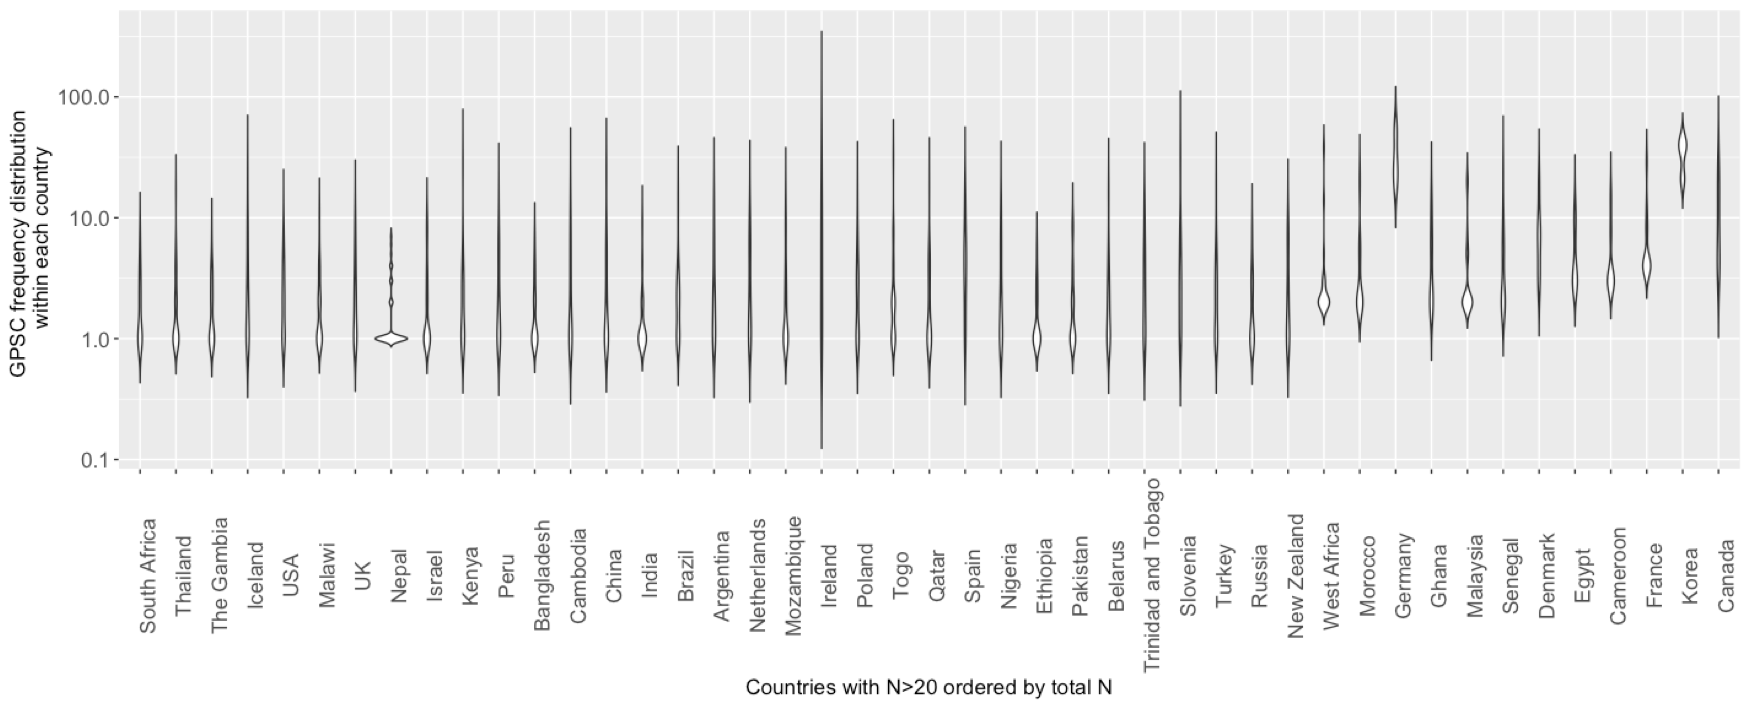
\includegraphics[width=\textwidth]{08MAR21_gpscfreqDistribution.png}
    \caption{Caption}
    \label{fig:gpscfreqdist}
\end{figure} 
Several of these high frequency GPSCs are consistent across countries while low frequency GPSCs are more varied. This may be a result of geographically varied sampling strategies depending upon whether the samples were carriage or disease, the age sampled, co-existing conditions in the individuals being sampled, among other things [PAPERS SHOWING DIFFERENT GPSCS/CCS/SEROTYPES BY AGE DISEASE CARRIAGE ETC]. 
The high levels of diversity of the pneumococcus, comprising highly recombinatory genetic backbones and serotypes, entreats the question of spatial structure. Is the world a homogeneous soup of pneumococcal diversity, or is there variability in the range of these GPSCs with some restricted to geographic regions while others may maintain prevalence globally.  This is contingent on time, how recently have GPSCs diverged, and how long have they been circulating? Are there distinct differences in the population ecology in different geographic locations or are the differences we are empirically noting a result of bias in our datasets? 
The short range transmission dynamics are key to understanding how quickly it spreads and in turn how far. Rates of asymptomatic carriage in children under 5 range from 20-90\% with an inverse relationship to country income[CITEHIC] \cite{adegbolaCarriageStreptococcusPneumoniae2014}.  The high prevalence in children as well as the increased risk of adult carriage in households with children under 18 has led to the conclusion that children are the drivers of transmission\cite{almeidaDynamicsPneumococcalCarriage2020}. Carriage duration is estimated to be around 2 months but has been recorded for up to a year \cite{almeidaDynamicsPneumococcalCarriage2020,dubeLongitudinalCharacterizationNasopharyngeal2018}. [MORE CARRIAGE DURATION.] A meta-analysis of lower-middle income countries indicated a wide range of carriage rates in adults from 8-85\% \cite{adegbolaCarriageStreptococcusPneumoniae2014}. Another study undertaken in the UK indicates a carriage prevalence of 20-40\% in adults\cite{almeidaDynamicsPneumococcalCarriage2020} . Carriage rates in adults is an under investigated topic likely due to the focus on the individuals with the greatest burden of disease --- children <5. 
\textbf{TRANSMISSION } The pneumococcus colonizes mucosal surfaces in the upper respiratory tract, it promotes inflammation predominantly via pneumolysins which results in secretions and shedding. Close contact, co-occurrence with viral infections, and colder drier months all correlate with more likely transmission. The estimated generation time, time from infection to transmission, is estimated to be 1-2 months but is not well characterized. GPSCs carrying specific serotypes may be likely to be carried asymptomatically for a longer duration while others transmit more quickly. [CITE]
To truly determine the speed and breadth of pneumococcal transmission requires a good estimate of divergence times between pairs. Phylogenetic methods and the increasing availability of software to time resolve divergence makes this possible \cite{didelotBayesianInferenceAncestral2018,drummondBayesianEvolutionaryAnalysis2015}. A requirement of these methods is a time range that allows the branch length --- indicative of mutation rate --- to be 

\subsection{genome-recombination-pangenome}
\\ NOTES MUTATION RATE WITHIN HOST 5.3 snps/genome/year. weak correlation between the date of a strain’s isolation and its distance from the root of the tree (Pearson correlation, N = 222, R2 = 0.05, p = 0.001; Fig. S1), suggesting variation was primarily arising through incorporation of imported DNA and not through steady accumulation of base substitutions he rate at which base substitutions occur outside of recombinations suggests a mutation rate of 1.57 × 10−6 substitutions per site per year (95\% confidence interval 1.34-1.79 × 10−6)(https://www.ncbi.nlm.nih.gov/pmc/articles/PMC3648787/)T
\\This promiscuity is what facilitates the previously mentioned serotype switching, but it also allows exchange of many other genes 
his promiscuity allows constant adaptation to pressures such as vaccination, antimicrobial use, and variable numbers of available hosts. \\Work is ongoing to understand which NVTs emerge following PCV implementation on a country by country basis however, as has been demonstrated with the global dispersal of SARS-Cov-2 variants in 2020-2021, we are an interconnected globalized world. Introduction of a virulent pneumococcal strain has the potential to disturb the existing population ecology and spread. We currently don't have any estimates for long range transmission dynamics of \textit{Streptococcus pneumoniae} either within or between countries. 
1200words
\section{Aims}
My PhD is working towards elucidating the spatiotemporal dynamics of the pneumococcus. I began with characterization of an ancient streptococcal genome initially characterized as pneumococcus, with the intention of identifying its closest strain and beginning to understand which strains have persisted for thousands of years and which have recently expanded. 
200 words
\section{Methods}
\subsection{Characteristics of an ancient streptococcal genome}
\subsection{Spatiotemporal dynamics of the pneumococcus in South Africa}
500 words
\section{Results}
1000 words
\section{Discussion}
900 words
\section{Future Work}
1000 words
\section{Gantt Chart}
\printbibliography
\end{document}
